%\documentclass[landscape,a0b,final,a4resizeable]{a0poster}
%\documentclass[portrait,a0b,final]{a0poster}
\documentclass[portrait,a0b,final]{a0poster}
%\documentclass[orientation=landscape,size=a0,scale=1,final]{a0poster}
%\documentclass[final]{beamer}
%\mode<presentation>
%{
%\usepackage[orientation=landscape,size=a0,scale=1.4,debug]{beamerposter}
%\documentclass[portrait,a0b,final,a4resizeable]{a0poster}
%\documentclass[portrait,a0b,final]{a0poster}
%%% Option "a4resizeable" makes it possible ot resize the
%   poster by the command: psresize -pa4 poster.ps poster-a4.ps
%   For final printing, please remove option "a4resizeable" !!

%\usepackage[ruled,lined]{algorithm2e}
%\def\algorithmautorefname{Algorithm}
%\SetKwIF{If}{ElseIf}{Else}{if}{then}{else if}{else}{endif}

\usepackage{amssymb,amsfonts,amsmath,latexsym,amsthm}
\usepackage[usenames,dvipsnames]{color}
\usepackage{enumitem}
%\theoremstyle{plain}
\newtheorem{theorem}{Theorem}[section]
\newtheorem{corollary}[theorem]{Corollary}
\newtheorem{lemma}[theorem]{Lemma}
\newtheorem{proposition}[theorem]{Proposition}
\newtheorem{condition}[theorem]{Condition}
\newtheorem{algorithm}[theorem]{Algorithm}

\newcommand{\clusters}{\bm{\kappa}}
\newcommand{\cluster}[1]{\kappa_{#1}}
\newcommand{\sizes}{\bm{\mu}}
\newcommand{\size}[1]{\mu_{#1}}
\newcommand{\edist}{\bm{\gamma}}
\newcommand{\shape}{\eta}
\newcommand{\rate}{s}
\newcommand{\betaA}{u}
\newcommand{\betaB}{v}


% Probability distributions
\DeclareMathOperator*{\Exp}{Exp}
\DeclareMathOperator*{\TExp}{TExp}
\DeclareMathOperator*{\Bernoulli}{Bernoulli}
\DeclareMathOperator*{\Beta}{Beta}
\DeclareMathOperator*{\Ga}{Gamma}
\DeclareMathOperator*{\TGamma}{TGamma}
\DeclareMathOperator*{\Poisson}{Poisson}
\DeclareMathOperator*{\Binomial}{Binomial}
\DeclareMathOperator*{\NormalGamma}{NormalGamma}
\DeclareMathOperator*{\InvGamma}{InvGamma}
\DeclareMathOperator*{\Cauchy}{Cauchy}
\DeclareMathOperator*{\Uniform}{Uniform}
\DeclareMathOperator*{\Gumbel}{Gumbel}
\DeclareMathOperator*{\Pareto}{Pareto}
\DeclareMathOperator*{\Mono}{Mono}
\DeclareMathOperator*{\Geometric}{Geometric}
\DeclareMathOperator*{\Dirichlet}{Dirichlet}
\DeclareMathOperator*{\Categorical}{Categorical}
\DeclareMathOperator*{\Multinomial}{Multinomial}
\DeclareMathOperator*{\DirichletMultinomial}{DirichletMultinomial}

% Math operators
\DeclareMathOperator*{\argmin}{arg\,min}
\DeclareMathOperator*{\argmax}{arg\,max}
\DeclareMathOperator*{\Cov}{Cov}
\DeclareMathOperator*{\diag}{diag}
\DeclareMathOperator*{\median}{median}
\DeclareMathOperator*{\Vol}{Vol}
\DeclareMathOperator*{\PCM}{PCM}

% Math characters
\newcommand{\R}{\mathbb{R}}
\newcommand{\Z}{\mathbb{Z}}
\newcommand{\E}{\mathbb{E}}
\renewcommand{\Pr}{\mathbb{P}}
\newcommand{\I}{\mathds{1}}
\newcommand{\V}{\mathbb{V}}

\newcommand{\A}{\mathcal{A}}
\newcommand{\C}{\mathcal{C}}
\newcommand{\D}{\mathcal{D}}
\newcommand{\Hcal}{\mathcal{H}}
\newcommand{\M}{\mathcal{M}}
\newcommand{\N}{\mathcal{N}}
\newcommand{\X}{\mathcal{X}}
\newcommand{\Zcal}{\mathcal{Z}}
\renewcommand{\P}{\mathcal{P}}

\newcommand{\T}{\mathtt{T}}
\renewcommand{\emptyset}{\varnothing}

\newcommand{\g}{\,|\,}



\usepackage[usenames,dvipsnames]{xcolor}
%\usepackage{tkz-berge}
%\usetikzlibrary{fit,shapes}

\usepackage{calc}
%%
%% The tikz package is used for doing the actual drawing.
\usepackage{tikz}

\usepackage{caption}

%%
%% In order to be able to put arrowheads in the middle of directed edges, we need an extra library.
\usetikzlibrary{decorations.markings}
%%
%% The next line says how the "vertex" style of nodes should look: drawn as small circles.
\tikzstyle{vertex}=[circle, draw, inner sep=0pt, minimum size=6pt]
%%
%% Next, we make a \vertex command as a shorthand in place of \node[vertex} to get that style.
\newcommand{\vertex}{\node[vertex]}
%%
%% Finally, we declare a "counter", which is what LaTeX calls an integer variable, for use in
%% the calculations of angles for evenly spacing vertices in circular arrangements.
\newcounter{Angle}



\renewcommand{\baselinestretch}{1.2}
%\usepackage[usenames,dvipsnames]{xcolor}
%\thispagestyle{empty}


\usepackage{epsfig,bm}
\usepackage{multicol}
\usepackage{pstricks,pst-grad}
\usepackage{amssymb,amsmath,amstext,graphicx,amsopn,amsfonts,bm}
\newcommand{\draw}{\stackrel{\text{draw}}{\sim}}

 
 

\usepackage[sort&compress]{natbib}
\bibpunct{(}{)}{;}{a}{}{,}
%\newtheorem{theorem}{Theorem}
%%%%%%%%%%%%%%%%%%%%%%%%%%%%%%%%%%%%%%%%%%%
% Definition of some variables and colors
%\renewcommand{\rho}{\varrho}
%\renewcommand{\phi}{\varphi}
\setlength{\columnsep}{3cm}
\setlength{\columnseprule}{2mm}
\setlength{\parindent}{0.0cm}

\newcommand{\indep}{\stackrel{\text{indep}}{\sim}}
\newcommand{\cas}{\buildrel \textrm{\scriptsize a.s.} \over
  \longrightarrow}
\newcommand{\cd}{\buildrel d \over \longrightarrow}
\newcommand{\cp}{\buildrel P \over \longrightarrow}
%\newcommand{\R}{\mathbb{R}}
\newcommand{\hatbb}{\boldsymbol{\hat{b}}}
\newcommand{\hatbB}{\boldsymbol{\hat{B}}}
\newcommand{\hatbd}{\boldsymbol{\hat{d}}}
\newcommand{\commentt}[1]{}
\newcommand{\myvfil}[1]{\vskip 0pt plus #1fill}
% \renewcommand{\upsilon}{v}
\newcommand{\lik}{\ell_y(\theta)}
\newcommand{\likil}{\ell_y(\theta_i^{(l)})}
\newcommand{\hd}{\hfill$\diamondsuit$}
\newcommand{\aaa}{\epsilon}
\newcommand{\lt}{\left}
\newcommand{\rt}{\right}
\newcommand{\mbi}{\max_{1 \leq i \leq m} \bxi'\bb}
\newcommand{\bs}{B_{i*}}
\newcommand{\bi}{B_{i}}
\newcommand{\that}        {\mbox{$\hat{\boldsymbol{\theta}}$}}
\newcommand{\utheta}        {\mbox{$\boldsymbol{\theta}$}}
\newcommand{\thhj}{\hat{\theta}_j}
\newcommand{\thhij}{\hat{\theta}_{ij}}
\newcommand{\thiHB}{\hat{\theta}_i^{HB}}
\newcommand{\thih}{\hat{\theta}_i^H}
\newcommand{\thit}{\tilde{\theta}_i^H}


\newcommand{\tr}{\text{tr}}
\newcommand{\btt}{\boldsymbol{\theta}}

\newcommand{\ttt}{\boldsymbol{t}}
\newcommand{\bhat}{\boldsymbol{\hat{\beta}}}
\newcommand{\thb}{\bar{\theta}}
\newcommand{\bx}{\boldsymbol{x}}
\newcommand{\bv}{\boldsymbol{v}}
\newcommand{\bu}{\boldsymbol{u}}
\newcommand{\ur}{\boldsymbol{r}}
\newcommand{\uphi}{\boldsymbol{\phi}}
\newcommand{\uone}{\boldsymbol{1}}
\newcommand{\ue}{\boldsymbol{e}}
\newcommand{\uc}{\boldsymbol{c}}
\newcommand{\bbi}{\boldsymbol{b}_i}
\newcommand{\uw}{\boldsymbol{w}}
\newcommand{\bz}{\boldsymbol{z}}
\newcommand{\be}{\boldsymbol{e}}
\newcommand{\by}{\boldsymbol{y}}
\newcommand{\utt}{\boldsymbol{t}}
\newcommand{\bzero}{\boldsymbol{0}}
\newcommand{\bl}{\boldsymbol{l}}
\newcommand{\util}{\boldsymbol{\tilde{u}}}
\newcommand{\btil}{\boldsymbol{\tilde{\beta}}}
\newcommand{\btils}{\boldsymbol{\tilde{\beta}_*}}
%\newcommand{\bm}{\boldsymbol{m}}
\newcommand{\btilf}{(X'V^{-1}X)^{-1}X'V^{-1}\that}
\newcommand{\btilfs}{(X'V_*^{-1}X)^{-1}X'V_*^{-1}\that}
\newcommand{\bxij}{\boldsymbol{x_{ij}}}
\newcommand{\bxj}{\boldsymbol{x}_j}
\newcommand{\bei}{\boldsymbol{e_{i}}}
\newcommand{\bej}{\boldsymbol{e_{j}}}
\newcommand{\bbary}{\boldsymbol{\bar{y}}}
\newcommand{\thet}{\boldsymbol{\theta}}


\newcommand{\bX}       {\mbox{$\boldsymbol{X}$}}
\newcommand{\lam}       {\mbox{$\boldsymbol{\Lambda}$}}
\newcommand{\lao}       {\mbox{$\lambda_{1i}$}}
\newcommand{\lat}       {\mbox{$\lambda_{2}$}}
\newcommand{\latt}       {\mbox{$\lambda_{3i}$}}


\newcommand{\vv}        {V^{-1}}
\newcommand{\vs}        {V^{-1}_*}
\newcommand{\sig}        {\Sigma}
\newcommand{\sm}        {\sqrt{m}}
\newcommand{\thi}        {\theta_i}
\newcommand{\thhi}        {\mbox{$\hat{\theta}_i$}}
\newcommand{\thhk}        {\mbox{$\hat{\theta}_k$}}
\newcommand{\thho}        {\mbox{$\hat{\theta}_1$}}
\newcommand{\thhm}        {\mbox{$\hat{\theta}_m$}}
\newcommand{\thj}        {\mbox{$\hat{\theta}_j$}}
\newcommand{\thij}        {\mbox{$\hat{\theta}_{ij}$}}

\newcommand{\thk}        {\mbox{$\hat{\theta}_k$}}
\newcommand{\tij}       {\mbox{$\theta_{ij}$}}
\newcommand{\thbb}        {\mbox{$\hat{\theta}^B$}}
\newcommand{\thbi}        {\mbox{$\hat{\theta}_i^\text{B}$}}
\newcommand{\thbis}        {\mbox{$\hat{\theta}_{i*}^B$}}
\newcommand{\thebis}        {\mbox{$\hat{\theta}_{i*}^{\text{EB}}$}}
\newcommand{\thebjs}        {\mbox{$\hat{\theta}_{j*}^{EB}$}}
\newcommand{\thbj}        {\mbox{$\hat{\theta}_j^B$}}
\newcommand{\thbjs}        {\mbox{$\hat{\theta}_{j*}^B$}}
\newcommand{\thbk}        {\mbox{$\hat{\theta}_k^B$}}
\newcommand{\htijb}        {\mbox{$\hat{\theta}_{ij}^B$}}
\newcommand{\thebi}       {\mbox{$\hat{\theta}_i^{\text{EB}}$}}
\newcommand{\thebj}       {\mbox{$\hat{\theta}_j^{EB}$}}
\newcommand{\theblupi}    {\mbox{$\hat{\theta}_i^{\text{EBM1}}$}}
\newcommand{\theblupis}       {\mbox{$\hat{\theta}_{i*}^{\text{EBM1}}$}}

\newcommand{\thbiw}       {\mbox{$\bar{\hat{\theta}}_{iw}^B$}}
\newcommand{\tbw}       {\mbox{$\bar{\theta}_{w}$}}
\newcommand{\thww}       {\mbox{$\bar{\hat{\theta}}_{w}$}}
\newcommand{\thw}       {\mbox{$\bar{\hat{\theta}}_{w}^B$}}
\newcommand{\tbiw}       {\mbox{$\bar{\theta}_{iw}$}}
\newcommand{\thbariw}     {\mbox{$\bar{\hat{\theta}}_{iw}^{B}$}}
\newcommand{\thbarw}     {\mbox{$\bar{\hat{\theta}}_{w}^{B}$}}
\newcommand{\thbarwb}     {\mbox{$\bar{\hat{\theta}}_w^{B}$}}
\newcommand{\thbarwbs}     {\mbox{$\bar{\hat{\theta}}_{w*}^{B}$}}
\newcommand{\thbarweb}     {\mbox{$\bar{\hat{\theta}}_w^{\text{EB}}$}}
\newcommand{\thbarwebs}     {\mbox{$\bar{\hat{\theta}}_{w*}^{EB}$}}
\newcommand{\se}     {\mbox{$\sigma_{ei}^2$}}
\newcommand{\su}     {\mbox{$\sigma_u^2$}}
\newcommand{\sbb}     {\mbox{$\sigma_b^2$}}
\newcommand{\sut}     {\mbox{$\tilde{\sigma}_u^2$}}
\newcommand{\suh}     {\mbox{$\hat{\sigma}_u^2$}}
\newcommand{\sus}     {\mbox{${\sigma}_u^{*2}$}}
\newcommand{\sust}     {\mbox{$\tilde{\sigma}_u^{*2}$}}
%\newcommand{\btil}     {\mbox{$(X'V^{-1}X)^{-1}X'V^{-1}\boldface{\theta}$}}
\newcommand{\hvis}     {\mbox{$\boldsymbol{x}_i'(X'V^{-1}_*X)^{-1}\boldsymbol{x}_i$}}
\newcommand{\hvi}     {\mbox{$\boldsymbol{x}_i'(X'V^{-1}X)^{-1}\boldsymbol{x}_i$}}
\newcommand{\hij}     {\mbox{$\boldsymbol{x}_i'(X'X)^{-1}\boldsymbol{x}_j$}}
\newcommand{\hvk}     {\mbox{$\boldsymbol{x}_k'(X'V^{-1}X)^{-1}\boldsymbol{x}_k$}}
\newcommand{\hj}     {\max_{1\leq j \leq m} h_j}
\newcommand{\hi}     {\max_{1\leq i \leq m} h_i}
\newcommand{\hk}     {\mbox{$\boldsymbol{x}_k'(X'X)^{-1}\boldsymbol{x}_k$}}
\newcommand{\hvik}     {\mbox{$\boldsymbol{x}_i'(X'V^{-1}X)^{-1}\boldsymbol{x}_k$}}
\newcommand{\hii}     {\mbox{$\boldsymbol{x}_i'(X'X)^{-1}\boldsymbol{x}_i$}}
%\newcommand{\bt}     {\mbox{$\tilde{\bm{\beta}}$}}
\newcommand{\ut}     {\mbox{$\tilde{\boldsymbol{u}}$}}
\newcommand{\uts}     {\mbox{$\tilde{\boldsymbol{u}}_*$}}
\newcommand{\ub}     {\mbox{${\boldsymbol{u}}$}}
\newcommand{\bb}     {\mbox{${\boldsymbol{\beta}}$}}
\newcommand{\li}     {\mbox{${\lambda_i}$}}
\newcommand{\lj}     {\mbox{${\lambda_j}$}}
\newcommand{\lk}     {\mbox{${\lambda_k}$}} 
\newcommand{\co}     {\text{Cov}}
\newcommand{\lp}     {\left(}
\newcommand{\rp}     {\right)}
\newcommand{\lb}     {\left\{}
\newcommand{\rb}     {\right\}}
%\newcommand{\g}     {\mbox{$X(X'V^{-1}X)^{-1}X'$}}
\newcommand{\bxi}{\boldsymbol{x}_i}
\newcommand{\bci}{\boldsymbol{c}_i}
\newcommand{\bgi}{\boldsymbol{g}_i}
\newcommand{\bxk}{\boldsymbol{x}_k}
\newcommand{\byi}{\boldsymbol{y}_i}
\newcommand{\bzi}{\boldsymbol{z}_i}
\newcommand{\bt}{\boldsymbol{\tilde{\beta}}}
\newcommand{\lai}     {\lambda_i}
\newcommand{\gai}     {\gamma_i}

\newcommand{\cov}     {\text{Cov}}

%%slides
\newcommand{\hti}       {\hat{\theta}_i} 
\newcommand{\hto}       {\hat{\theta}_1}
\newcommand{\htm}       {\hat{\theta}_m}  
\newcommand{\htbi}       {\hat{\theta}_i^B} 
\newcommand{\bhto}   	   {\hat{\boldsymbol{\theta}}^{(1)}}
\newcommand{\bhtr}   	   {\hat{\boldsymbol{\theta}}^{(r)}}
\newcommand{\bhtPB}   	   {\hat{\boldsymbol{\theta}}^{(PB)}}
\newcommand{\bhttwo}   	   {\hat{\boldsymbol{\theta}}^{(2)}}

\newcommand{\bhtw}   	   	   {\bar{\hat{\theta}}_w}

\newcommand{\bhtwb}   	   {\bar{\hat{\theta}}_w^B}
\newcommand{\bhtwbb}   	  {\bar{\hat{\bm{\theta}}}_w^B}

%\newcommand{\bt}			{\bm{\theta}}
%\newcommand{\be}			{\bm{e}}
%\newcommand{\btt}			{\bm{t}}
\newcommand{\bW}			{\boldsymbol{W}}
\newcommand{\bO}			{\boldsymbol{\Omega}}
\newcommand{\br}			{\boldsymbol{r}}


\newcommand{\bbmo}   	  	{\hat{\boldsymbol{\theta}}^{BM1}}
\newcommand{\bht}   	  	{\hat{\thet}^B}
%\newcommand{\bbt}   	  	{\hat{\bt}}
\newcommand{\BM}   	  {\hat{\theta}^{BM1}}
\newcommand{\bmo}   	  {\hat{\theta}_1^{BM1}}
\newcommand{\bmi}   	  {\hat{\theta}_i^{BM1}}
\newcommand{\bmov}   	  {\hat{\bt}_1^{BM1}}
\newcommand{\bmm}   	  {\hat{\theta}_m^{BM1}}
\newcommand{\bhmbm}   	  {\hat{\theta}^{MBM}}
\newcommand{\bhmbmb}   	  {\hat{\boldsymbol{\theta}}^{MBM}}
\newcommand{\swtbm}   	  {\sum_{i=1}^m w_i\bmi}
\newcommand{\bmtwo}   	  {\hat{\theta}_i^{BM2}}

\newcommand{\ma}     {\max_{1 \leq i \leq m}}

%%
\newcommand{\sustt}     {\mbox{${\hat{\sigma}}_u^{*2}$}}
\newcommand{\thebs}     {\hat{\theta}_i^{\text{EB*}}}
\newcommand{\btheta}{\boldsymbol{\theta}}
\newcommand{\bthat}{\hat{\boldsymbol{\theta}}^B}
\newcommand{\bw}{\boldsymbol{w}}


%%%%%%%%%%%%%%%%%%%%%%%%%%%%%%%%%%%%%%%%%%%%%%%%%%%%
%%%               Background                     %%%
%%%%%%%%%%%%%%%%%%%%%%%%%%%%%%%%%%%%%%%%%%%%%%%%%%%%

\newcommand{\background}[3]{
  \newrgbcolor{cgradbegin}{#1}
  \newrgbcolor{cgradend}{#2}
  \psframe[fillstyle=gradient,gradend=cgradend,
  gradbegin=cgradbegin,gradmidpoint=#3](0.,0.)(1.\textwidth,-1.\textheight)
}



%%%%%%%%%%%%%%%%%%%%%%%%%%%%%%%%%%%%%%%%%%%%%%%%%%%%
%%%                Poster                        %%%
%%%%%%%%%%%%%%%%%%%%%%%%%%%%%%%%%%%%%%%%%%%%%%%%%%%%

\newenvironment{poster}{
  \begin{center}
  \begin{minipage}[c]{0.98\textwidth}
}{
  \end{minipage}
  \end{center}
}



%%%%%%%%%%%%%%%%%%%%%%%%%%%%%%%%%%%%%%%%%%%%%%%%%%%%
%%%                pcolumn                       %%%
%%%%%%%%%%%%%%%%%%%%%%%%%%%%%%%%%%%%%%%%%%%%%%%%%%%%

\newenvironment{pcolumn}[1]{
  \begin{minipage}{#1\textwidth}
  \begin{center}
}{
  \end{center}
  \end{minipage}
}



%%%%%%%%%%%%%%%%%%%%%%%%%%%%%%%%%%%%%%%%%%%%%%%%%%%%
%%%                pbox                          %%%
%%%%%%%%%%%%%%%%%%%%%%%%%%%%%%%%%%%%%%%%%%%%%%%%%%%%

\newrgbcolor{lcolor}{0. 0. 0.80}
\newrgbcolor{gcolor1}{1. 1. 1.}
\newrgbcolor{gcolor2}{.80 .80 1.}

\newcommand{\pbox}[4]{
\psshadowbox[#3]{
\begin{minipage}[t][#2][t]{#1}
#4
\end{minipage}
}}



%%%%%%%%%%%%%%%%%%%%%%%%%%%%%%%%%%%%%%%%%%%%%%%%%%%%
%%%                myfig                         %%%
%%%%%%%%%%%%%%%%%%%%%%%%%%%%%%%%%%%%%%%%%%%%%%%%%%%%
% \myfig - replacement for \figure
% necessary, since in multicol-environment
% \figure won't work

\newcommand{\myfig}[3][0]{
\begin{center}
  \vspace{.25cm}
  \includegraphics[width=#3\hsize,angle=#1]{#2}
  \nobreak\medskip
\end{center}}



%%%%%%%%%%%%%%%%%%%%%%%%%%%%%%%%%%%%%%%%%%%%%%%%%%%%
%%%                mycaption                     %%%
%%%%%%%%%%%%%%%%%%%%%%%%%%%%%%%%%%%%%%%%%%%%%%%%%%%%
% \mycaption - replacement for \caption
% necessary, since in multicol-environment \figure and
% therefore \caption won't work

%\newcounter{figure}
\setcounter{figure}{1}
\newcommand{\mycaption}[1]{
  \vspace{0.25cm}
  \begin{quote}
    {{\sc Figure} \arabic{figure}: #1}
  \end{quote}
  \vspace{0.25cm}
  \stepcounter{figure}
}




%%%%%%%%%%%%%%%%%%%%%%%%%%%%%%%%%%%%%%%%%%%%%%%%%%%%%%%%%%%%%%%%%%%%%%
%%% Begin of Document
%%%%%%%%%%%%%%%%%%%%%%%%%%%%%%%%%%%%%%%%%%%%%%%%%%%%%%%%%%%%%%%%%%%%%%

\begin{document}

\background{1. 1. 1.}{1. 1. 1.}{0.5}
\vspace*{1.5cm}

\newrgbcolor{lightblue}{0. 0. 0.80}
\newrgbcolor{white}{1. 1. 1.}
\newrgbcolor{whiteblue}{.80 .80 1.}


\begin{poster}

%%%%%%%%%%%%%%%%%%%%%
%%% Header
%%%%%%%%%%%%%%%%%%%%%
\begin{center}
\begin{pcolumn}{0.98}
\pbox{0.95\textwidth}{}{linewidth=2mm,framearc=0.3,linecolor=lightblue,fillstyle=gradient,gradangle=0,gradbegin=white,
gradend=whiteblue,gradmidpoint=1.0,framesep=1em}{

%%%% Unisiegel
%\begin{minipage}[c][9cm][c]{0.1\textwidth}
%  \begin{center}
%      \includegraphics[width=10cm,angle=0]{SOE_logo.eps}
%  \end{center}
%\end{minipage}
%%% Titel
\begin{minipage}[c][7.2cm][c]{\textwidth}
  \begin{center}
    %{\sc \huge \bf Will the real Alan Gelfand Please Stand up: A Bayesian Nonparametric Method for Record Linkage 
    {\sc \huge \bf Flexible Models for Microclustering with Application to Entity Resolution
}\\[10mm]
%    {\sc \huge of Benchmarked Empirical Bayes Estimators\bf  }\\[10mm]
    {\Large Brenda Betancourt,${}^{1}$ Giacomo Zanella,${}^{2}$ Hanna Wallach,${}^{3}$  Jeffrey W. Miller,${}^{4}$ Abbas Zaidi,${}^{1}$ and Rebecca C. Steorts${}^{1}$      \\ [7.5mm]
Duke University,${}^{1}$, Bocconi University,${}^{2}$
 Microsoft Research,${}^{3}$ and Harvard University${}^{4}$ }
  \end{center}
\end{minipage}
%%%% GK-Logo
%\begin{minipage}[c][9cm][c]{0.1\textwidth}
%  \begin{center}
%    \reflectbox{\includegraphics[width=7cm,angle=0]{slug.eps}}
%  \end{center}
%\end{minipage}

}
\end{pcolumn}
\end{center}


\vspace*{1cm}

%%%%%%%%%%%%%%%%%%%%%
%%% Content
%%%%%%%%%%%%%%%%%%%%%
%%% Begin of Multicols-Enviroment
\begin{multicols}{3}

%%% Parametric Model
\vspace{.75cm}
\begin{center}
  \pbox{0.8\columnwidth}{}{linewidth=2mm,framearc=0.1,linecolor=lightblue,fillstyle=gradient,
    gradangle=0,gradbegin=white,gradend=whiteblue,gradmidpoint=1.0,framesep=1em}{
    \begin{center}
      {\large \bf Summary}
    \end{center}
  }
\end{center}
\vspace{.65cm}

\begin{itemize}

\item Many models  assume the number of data points in each cluster grows linearly with the total number of data points.
\item Examples include infinitely exchangeable clustering processes. 
\item Entity resolution: the size of each cluster is often unrelated to the size of the data set.
\item Requires models that yield clusters whose sizes grow sublinearly with the size of the data set.
%\item Solution: The microclustering property and a new proposed model.
\end{itemize}

%\item We could merge 


  \begin{center}
      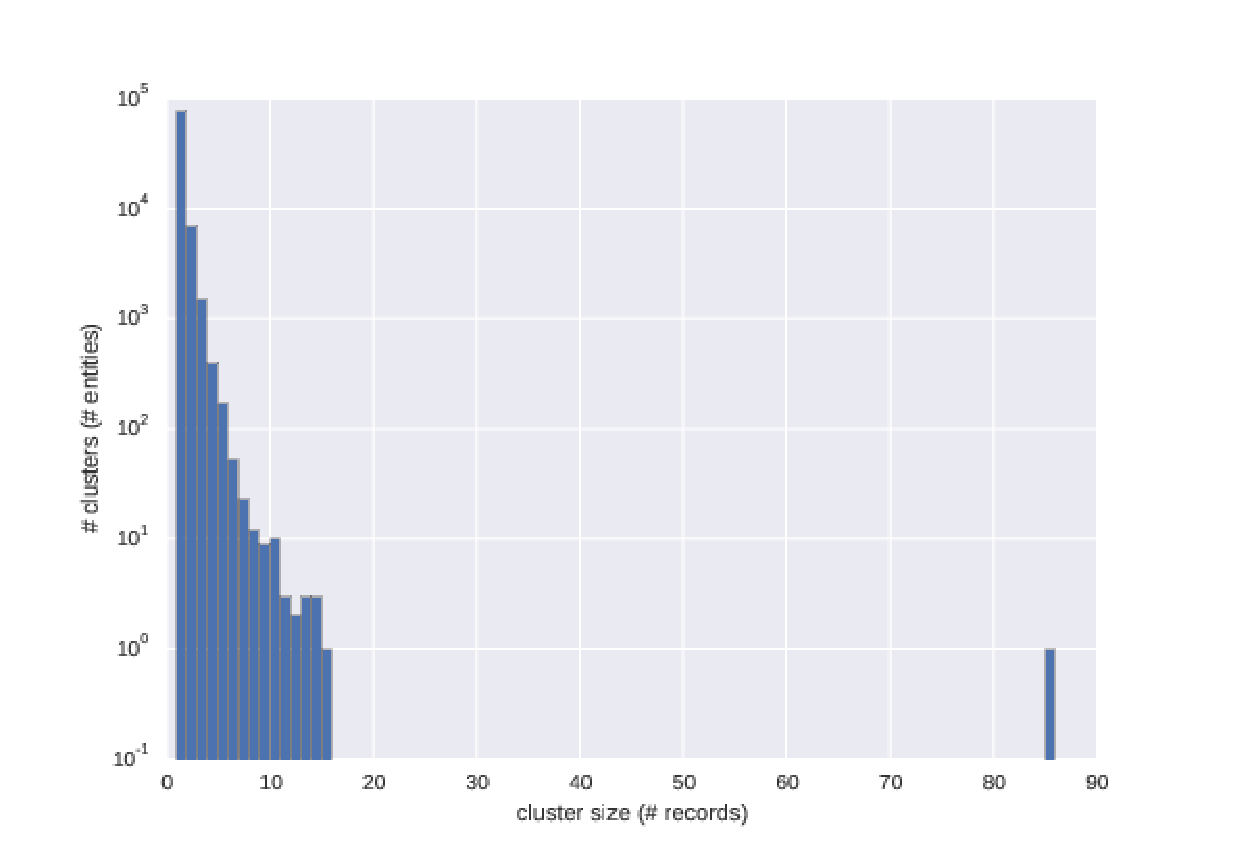
\includegraphics[width=0.15\textwidth]{donors_real.eps}
%      \includegraphics[width=0.3\textwidth]{real_2.pdf}
        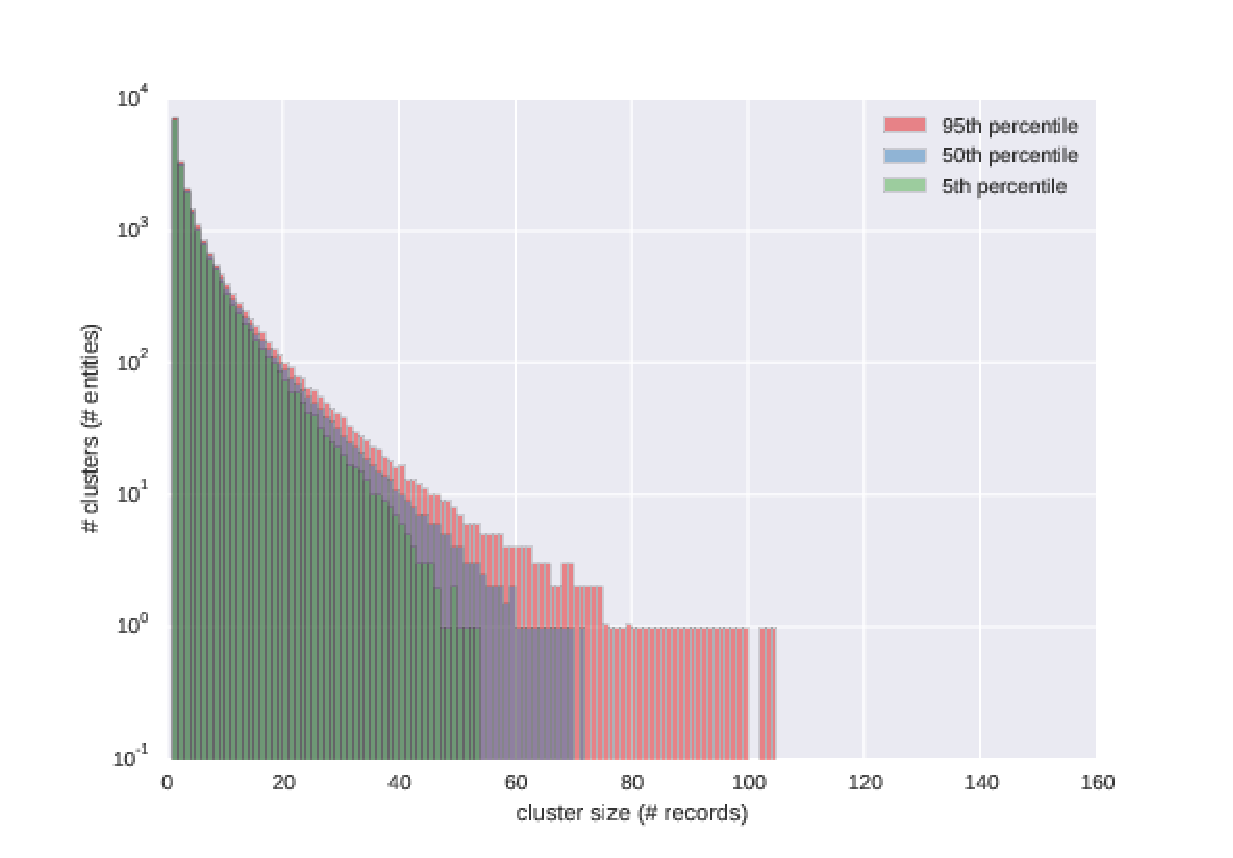
\includegraphics[width=0.15\textwidth]{donors_synthetic.eps}
         \mycaption{Two illustrations of the microclustering problem: (\emph{Left}) a
      histogram of the number of records per entity (i.e., cluster
      sizes) for a database of 100,000 campaign finance donations from
      2011--2012.  \emph{Right}: 
      A histogram of the cluster sizes generated from a Chinese restaurant process simulation with 
      concentration parameter 0.1. }
    \label{fig:small_clustering}
  \end{center}
  
  



\vspace*{1em}

%%% Motivating example
\begin{center}\pbox{0.8\columnwidth}{}{linewidth=2mm,framearc=0.1,linecolor=lightblue,fillstyle=gradient,gradangle=0,
gradbegin=white,gradend=whiteblue,gradmidpoint=1.0,framesep=1em}{\begin{center}{\large \bf Microclustering property }\end{center}}\end{center}
\vspace{.75cm}

\definecolor{myblue}{RGB}{80,80,160}
\definecolor{mygreen}{RGB}{80,160,80}


\begin{center}
\textbf{Traditional Clustering}
\end{center}
%\begin{itemize}
%\item Suppose we cluster $N$ data points using partition-based Bayesian clustering models. 
%We then place a prior over partitions of $[N].$
%\item Given a partition $C_N$ of $[N]$, we model $\bx$ in each part $c\in C_N$ as a joint distribution. 
%\item Mixture models are well known for such a partition based model, where $C_N$ is represented by cluster assignments $\bm{z} = (z_1,\ldots,z_N).$
%\item We can view the $\bz$ as 
%%the first $N$ elements of an infinite sequence 
%$z_1, z_2, \ldots$
%drawn from
%\begin{align}
%\bm{\pi} \sim H \quad \text{and} \quad z_1, z_2, \ldots \mid \bm{\pi} \stackrel{iid}{\sim} \bm{\pi}, \label{eqn:mixture}
%\end{align}
%where $\bm{\pi}$ is a vector of mixture weights with $\sum_c \pi_c =1$ and $\pi_c \geq 0.$
%\end{itemize}

%\begin{center}
%\textbf{Implications}
%\end{center}
%\begin{itemize}
%\item Equation \ref{eqn:mixture} implicitly defines a prior over partitions of N. 
%\item Any random partition $C_N$ of $\mathcal{N}$ induces a sequence of random partitions $(C_N : N = 1, 2, \ldots),$ where $C_N$ is a partition of $[N].$ 
%\item The cluster sizes in any such sequence obtained via equation \ref{eqn:mixture} grow
% linearly with $N$, since  $I(z_n =c)/N\stackrel{p}{\rightarrow} \pi_c$ as $N \rightarrow \infty.$
%\item Such linear growth is inappropriate for such tasks as entity resolution and other tasks that require the cluster sizes to grow sublinear with $N.$
%\end{itemize}

\begin{itemize}
\item A number of popular clustering applications assume priors on partitions such as the Dirichlet process and Pitman-Yor process distributions.
%\item These are all examples of a Kingman paintbox (Kingman 1978). % Kingman, J. F. C. (1978). ?The representation of partition structures.? Journal of the London Mathematical Society, 2(2): 374.
%\begin{center}
%\includegraphics[scale=0.5,angle=0]{pics/kingman}
%\mycaption{An example Kingman paintbox with 4 colors. A Kingman paintbox might have a countably infinite number of colors, a random number of colors, and/or random partition interval sizes. There are also 7 draws from the paintbox distribution here.}
%\end{center}
\item \emph{Any} infinitely exchangeable partition distribution on the positive integers has a Kingman paintbox representation.
\item Having a Kingman paintbox representation implies that the number of data points in each cluster grows (a.s.) linearly with the total number of data points $N$.
\item By contrast, in entity resolution (and other problems), we expect the size of the clusters to be small even for large datasets.
\end{itemize}

\vspace*{1em}

\begin{center}
\textbf{Microclustering}
\end{center}
A sequence of random partitions exhibits the \emph{microclustering property} if $M_N$ is $o_p(N)$, where $M_N \leq N$ is the size of the largest cluster in $C_N,$ where $C_N$ is a partition of $[N] = \{1,2, \ldots, N\}.$

\begin{itemize}
\item Equivalently, $M_N \,/\, N \rightarrow 0$ in probability as $N \rightarrow \infty$.
\item Microclustering requires sacrificing either (i) exchangeability or (ii) self-consistent marginalization of the partitions. 
\item Previous work Wallach et al. (2010) sacrificed (i); we sacrifice (ii).
\end{itemize}


%\begin{center}
%\textbf{Sacrificing Projectivity}
%\end{center}
%
%\begin{itemize}
%\item If a partition-based Bayesian clustering
%model is not finitely exchangeable, then inference will depend on the
%order of the data points. 
%\item For most applications, this consequence is
%undesirable---there is no reason to believe that the order of the data
%points is meaningful. 
%\item In contrast, if a model lacks projectivity, then
%the implied joint distribution over a subset of the data points in a
%data set will not be the same as the joint distribution obtained by
%modeling the subset directly.
%\item  In the context of entity resolution,
%sacrificing projectivity is a more natural and less restrictive choice
%than sacrificing finite exchangeability.
%\end{itemize}





\vspace{1em}

%\begin{itemize}
%\item No mixture model can satisfy the microclustering property (unless it's parameters vary with $N$) \citep{kingman78representation,aldous85exchangeability}
%\item By Kolmogorov's extension theorem, a sequence of random partitions corresponds to an an exchangeable random partition of N when (a) each $C_N$ is exchangeable and (b) the sequence is consistent in distribution.
%\item To obtain a non trivial model exhibiting the microclustering property, we must sacrifice (a) or (b). We sacrifice (b) since \cite{wallach10alternative} sacrificed (a). 
%\end{itemize}


%\vspace*{1em}






%%% LDA Like Model
%\vspace{.75cm}
\begin{center}
  \pbox{0.8\columnwidth}{}{linewidth=2mm,framearc=0.1,linecolor=lightblue,fillstyle=gradient,
    gradangle=0,gradbegin=white,gradend=whiteblue,gradmidpoint=1.0,framesep=1em}{
    \begin{center}
      {\large \bf Flexible Models for Microclustering}
    \end{center}
  }
\end{center}
\vspace{.65cm}

\begin{center}
\textbf{Notation}
\end{center}

\begin{itemize}
\item $K$:  number of clusters (random).
\item $N_k, \; k=1,\ldots K$: size of the $k$th cluster. 
\item $N = \sum_{k=1}^K N_k$: total number of data points.
\item $z_n, \; n=1,\ldots N$: cluster assignment of the $n$th data point.
\end{itemize}

Define
\begin{equation}
  K \sim \clusters \quad \textrm{and} \quad
 N_1,\ldots, N_K \mid K\,\stackrel{iid}\sim  \sizes.
\label{eq:FMMC}
\end{equation}
where $\clusters=(\cluster{1},\cluster{2},\dots)$ and $\sizes=(\size{1},\size{2},\dots)$ are probability distributions on $\{1,2,\ldots\}$. Given $N_1, \ldots, N_K$, generate 
$z_1, \ldots, z_N$ by drawing a vector uniformly at random from the
set of permutations of 
$$(\underbrace{1,\ldots,1}_\text{$N_1$
  times},\underbrace{2,\ldots,2}_\text{$N_2$
  times},\ldots\ldots,\underbrace{K,\ldots,K}_\text{$N_K$ times}).$$
  


\vspace*{1em}
 
\begin{center}
\textbf{NBNB Model}
\end{center}  
  
Suppose that we allow 
\begin{align*}
K \sim \text{Neg-Bin}(a,q)
\quad \textrm{and} \quad
N_1,\ldots, N_k \mid K \sim \text{Neg-Bin}(r,p),
\end{align*}
%where $\text{Neg-Bin}(a,q)$ and $\text{Neg-Bin}(r,p)$ are Negative Binomial distributions truncated on $\{1,2,\dots\}$. 
Note
\begin{itemize}
\item $a$ and $q$ are assumed to be known.
\item $r$ and $p$ are sampled from
Gamma and Beta priors.
%
%$r  \sim \text{Gamma}(\shape_r, \rate_r)$ and 
%$p  \sim \text{Beta}(\betaA_p,\betaB_p)$
%for some fixed $\shape_r$, $\rate_r$, $\betaA_p$ and $\betaB_p$.
\end{itemize}
We call the resulting marginal distribution of $C_N$ the \textcolor{blue}{NegBin-NegBin (NBNB)} model.
 
%Letting K denote the number of ``potential" (nonempty) clusters, we define
%\begin{align}
%  K \sim \textrm{NegBin}\,(a, q) \quad \textrm{and} \quad
% N_1, \ldots, N_K \g K \stackrel{iid}{\sim} \textrm{NegBin}\,(r, p),
%  \label{eqn:nbnb}
%\end{align}
%for $a, r \,>\, 0$ and $q, p \in (0, 1)$. 
%\begin{itemize}
%\item $K$ may be zero, as may
%some of $N_1, \ldots, N_K$. 
%\item Define $N = \sum_{k=1}^K N_k$ and,
%given $N_1, \ldots, N_K$, generate a set of cluster assignments $z1,\ldots, z_N$ by drawing a vector uniformly at random from the set of
%permutations of $$(\underbrace{1,\ldots,1}_\text{$N_1$
%  times},\underbrace{2,\ldots,2}_\text{$N_2$
%  times},\ldots\ldots,\underbrace{K,\ldots,K}_\text{$N_K$
%  times}).$$
%  \item Then  $z_1, \ldots, z_N$ induce a random partition
%$C_N$ of $[N]$.  We call the
%resulting marginal distribution of $C_N$ the NegBin--NegBin (NBNB)
%model. 
%%\item If $\mathcal{C}_N$ denotes the set of all possible partitions
%%of $[N]$, then $\bigcup_{N=1}^{\infty} \mathcal{C}_N$ is the set of
%%all possible partitions of $N$ for $N \in \mathbb{N}$.
%  \end{itemize}
%  
%  
%\textbf{Remark 1}:
%If we replace
%the negative binomials in (\ref{eqn:nbnb}) with Poissons, then
%we obtain a limiting special case of the NBNB model. We call this
%model the permuted Poisson sizes (PERPS) model.

\begin{center}
\textbf{NBD Model}
\end{center}

For a fully nonparametric approach, allow
\begin{align*}
K &\sim \text{Neg-Bin}(a,q)
\quad \textrm{and} \quad
N_1,\ldots, N_k \mid K \sim \bm{\mu},\\
\bm{\mu} &\sim \textcolor{red}{\text{Dirichlet}(\alpha, \sizes^{(0)})},
%\clusters = \text{Neg-Bin}(a,q) \quad \text{and} \quad \sizes \sim \textcolor{red}{\text{Dirichlet}(\alpha, \sizes^{(0)})},
\end{align*}
with fixed concentration parameter $\alpha>0$
and known base measure $$\sizes^{(0)}=(\mu^{(0)}_1,\mu^{(0)}_2,\cdots).$$
%with $\sum_{m=1}^\infty \mu^{(0)}_m=1$ and $\mu^{(0)}_m\geq 0$.
\begin{center}
\textbf{Sampling}
\end{center}

The reseating algorithm for the NBNB model is:
\begin{itemize}
\item for $n=1,\ldots N$, reassign element $n$ to
\begin{itemize}
\item an existing cluster $c\in C_{N}\setminus n$ with probability $\propto
|c|+r$
\item a new cluster with probability $\textcolor{red}{\propto (\textcolor{blue}{|C_N \setminus n|}+a)\beta r }.$
\end{itemize}
\end{itemize}
We can derive a similar reseating algorithm for the NBD model.

\vskip 1em

Compare to the reseating of the Chinese Restaurant Process (CRP):
\begin{itemize}
\item for $n=1,\ldots N$, reassign element $n$ to
\begin{itemize}
\item an existing cluster $c\in C_{N}\setminus n$ with probability $\propto
|c|$
\item a \textcolor{red}{new cluster} with probability $\textcolor{red}{\propto \alpha}.$
\end{itemize}
\end{itemize}
The parameter $\textcolor{red}{\alpha}$ induces the richer get richer behavior in the CRP. 
\vskip 1em

Main difference is the assignment to a new cluster depends on $K$ through the term $|C_N \setminus n|$. 

\vspace{-0.4cm}
\begin{center}
\includegraphics[width=0.3\textwidth]{figures/NBNB_NBD_microclustering}
\end{center}
\vspace{-1cm}
\mycaption{Empirical evidence suggesting that the NBNB (left) and NBD (right) models exhibit
 the microclustering property. }

%Conditional on $N$,
%the NBNB model implies that
%\begin{equation}
%  P(C_N \g N) \propto a^{(|C_N|)}\,\beta^{|C_N|} \, \prod_{c \in C_N}
%  r^{(|c|)},
%\end{equation}
%where $\beta = \left(q\,(1 - p)^r\right) \,/\, \left( 1 -
%q\,(1-p)^r\right)$. This leads a
%``reseating algorithm''---much like the Chinese restaurant process
%(CRP)---derived by sampling from $P(C_N \g N, C_N \!\setminus\! n)$,
%where $C_N \!\setminus\!  n$ is the partition obtained by removing
%element $n$ from $C_N$:
%\begin{itemize}
%\item for $n = 1,\ldots,N$, reassign element $n$ to
%  \begin{itemize}
%  \item an existing cluster $c \in C_N \!\setminus\! n$ with
%    probability $\propto |c| + r$,
%  \item a new cluster with probability $\propto
%    (|C_N \!\setminus\! n|+ a)\,\beta r$.
%  \end{itemize}
%\end{itemize}


\begin{itemize}
\item We can use the reseating algorithms to draw samples from $P(C_N \g N)$ but they do not 
produce exact samples like the CRP.
\item  When the NBNB or NBD
models are used as the prior in a partition-based clustering
model, the
resulting Gibbs sampling algorithm for $C_N$ is similar to this
algorithm accompanied by appropriate likelihood
terms. 
\item Unfortunately, incremental Gibbs sampling is slow for large data sets. 
\end{itemize}

\vspace*{1em}

\vspace{.25cm}\begin{center}\pbox{0.8\columnwidth}{}{linewidth=2mm,framearc=0.1,linecolor=lightblue,
fillstyle=gradient,gradangle=0,gradbegin=white,gradend=whiteblue,gradmidpoint=1.0,framesep=1em}
{\begin{center}{\large \bf Inference}\end{center}}\end{center}\vspace{.3cm}
\vspace*{1em}
In real world clustering tasks, data points $x_1, \ldots, x_n$ and $N$ are observed. 
Assume $x_{n, \ell}$ where:
\begin{itemize}
\item $n=1,\ldots N$ indexes how many records we observe.
\item $\ell=1,\ldots L$ indexes the categorical features within a record.
\end{itemize}
\vskip 1em
Let $\zeta:\bigcup_{N=0}^\infty(\mathcal C_{N}\times[N])\to\{1,2,\ldots\}$ be a function that maps a partition $C_{N}$ and a record~$x_{n,\ell}$ to its latent cluster assignment $z_n$.
%\footnote{For example,
%$
%\zeta\left(\{\{1,3,4\},\{2,5\},\{6\}\},4\right)=1$,
%$
%\zeta\left(\{\{1,3,4\},\{2,5\},\{6\}\},6\right)=3
%$
%because in this partition, record~$4$ is in cluster~$1$, while record~$6$ is in cluster~$3$.}
%Then
\begin{align*}
C_{N} &\sim \text{FMM}(\cdot) \\
z_n \mid C_{N} &= \zeta(C_{N}, n) \\
\bm{\theta}_{\ell,k} &\sim \text{Dirichlet}(\delta_\ell, \edist_\ell)\\
x_{n,\ell}\mid z_n,\bm{\theta}_{\ell,1},\bm{\theta}_{\ell,2},\dots&\sim \text{Multinomial}(\bm{\theta}_{\ell,z_n}),
\end{align*}

\begin{itemize}
\item The base measure $\edist_\ell$ is assumed known.
\item The concentration parameter $\delta_{\ell}  \sim \hbox{Gamma}(1,1)$.
\end{itemize}

\vspace*{1em}

\vspace{.25cm}\begin{center}\pbox{0.8\columnwidth}{}{linewidth=2mm,framearc=0.1,linecolor=lightblue,
fillstyle=gradient,gradangle=0,gradbegin=white,gradend=whiteblue,gradmidpoint=1.0,framesep=1em}
{\begin{center}{\large \bf Chaperones Algorithm}\end{center}}\end{center}\vspace{.3cm}
\vspace*{1em}

If we let $c_n \in C_N$ denote the cluster containing
element $n$, then each iteration consists of: 
\begin{enumerate}[label=\textbf{\arabic*.}]
\item Randomly choose two \emph{chaperones}, $i, j \in \{1, \ldots,
  N\}$ from a distribution $P(i, j \g x_1, \ldots, x_N)$ where the
  probability of $i$ and $j$ given $x_1, \ldots, x_N$ is greater
  than zero for all $i \neq j$. This distribution must be
  independent of the current state of the Markov chain $C_N$;
  however, crucially, it may depend on the observed data points
  $x_1, \ldots, x_N$.

\item Reassign each $n \in c_i \cup c_j$ by sampling from $P(C_N \g N,
  C_N \!\setminus\! n, c_i \cup c_j, x_1, \ldots, x_N)$.
\end{enumerate}

\vspace*{0.5em}

Step 2 is almost identical to the restricted
Gibbs moves found in existing split-merge algorithms (Jain and Neal, 2004), except that the chaperones $i$ and $j$ can also
change clusters, provided they do not abandon any of their children.
\vspace*{1em}

%\begin{center}
%\includegraphics[width=0.13\textwidth]{chaperones1}
%\end{center}
%\begin{center}
%\includegraphics[width=0.13\textwidth]{chaperones2}
%\end{center}
%\begin{center}
%\includegraphics[width=0.13\textwidth]{chaperones3}
%\end{center}
%\begin{center}
%\includegraphics[width=0.13\textwidth]{chaperones4}
%\end{center}





%\begin{center}
%\includegraphics{chaperones_v3.eps}
%\end{center}


\vspace{.25cm}\begin{center}\pbox{0.8\columnwidth}{}{linewidth=2mm,framearc=0.1,linecolor=lightblue,
fillstyle=gradient,gradangle=0,gradbegin=white,gradend=whiteblue,gradmidpoint=1.0,framesep=1em}
{\begin{center}{\large \bf Experiments}\end{center}}\end{center}\vspace{.3cm}
\vspace*{1em}

%\begin{center}
%\textbf{Assessing Model Fit}
%\end{center}
%\begin{itemize}
%\item We compare the NBNB and PERPS to several
%commonly used infinitely exchangeable models.
%%: mixtures of
%%finite mixtures (MFM)~\cite{miller15mixture}, DP mixtures, and PYP
%%mixtures. 
%\item We assess how well each model ``fits'' partitions typical of
%those arising in entity resolution and other tasks involving clusters
%whose sizes grow sublinearly with $N$.
%\item For simplicity and interpretability, we define
%the best parameter values for each model to be the values that
%maximize the probability of the observed partition.
%%\item We use two observed partitions -- ones simulated and one real. 
%\end{itemize}

\begin{center}
\textbf{The Data}
\end{center}
We assess how well each model ``fits" on simulated data based on three real data sets (medical data, official statistics data, and the Syrian conflict).
\begin{itemize}
\item Italy Data: Survey data from Italy with 74\% of data are singletons.
\item NLTCS5000: Sample from the National Long Term Care Survey (NLTCS) with 68\% singletons. 
\item Syria2000: Sample from Syrian conflict with 86\% singletons. 
\item Ground truth is known for all the above data sets, so we compare using such unique identifiers. 

%\item We use two observed partitions -- ones simulated and one real. 
%\item The simulated partition
%contains 5,000 elements, divided into 4,500 clusters. 
%\item Of these, 4,100
%are singleton clusters, 300 are clusters of size two, and 100 are
%clusters of size three. 
%\item In this paritition 91\% of the clusters are
%singletons.  
%\item The real partition comes from Survey on
%Household Income and Wealth, consisting of 789 records.
%\item Ground truth is available via unique
%identifiers based upon social security numbers; roughly 74\% of the
%clusters are singletons.
\end{itemize}

\begin{center}
\textbf{Evaluation Criterion}
\end{center}

\begin{itemize}
\item Consider four statistics: the number of
singleton clusters, the maximum cluster size, the mean cluster size,
and the 90\% quantile of cluster sizes. 
\item Consider three entity resolution metrics: estimated mean cluster size, False Negative Rate (FNR), and False Discovery Rate (FDR). 
\item Comparisons performed against the DP and PYP. 
%The intuition
%behind our approach is that if the observed value of a statistic is
%not well-supported by a given model, even with the MLE parameter
%values, then the model may not be appropriate for that type of data.
\end{itemize}

\begin{center}
\textbf{Results}
\end{center}

\begin{center}
\includegraphics[width=0.3\textwidth]{figures/Stats_Italy_upd}

\vspace{-1cm}

\includegraphics[width=0.3\textwidth]{figures/Stats_NLTCS5000_upd}

\vspace{-1cm}

\includegraphics[width=0.3\textwidth]{figures/Stats_Syria2000_upd}
\vspace{-0.5cm}
\mycaption{Top: Italy data. Middle: NLTCS5000. Bottom: Syria2000. The dashed horizontal line represents the true value of the statistic.}
\end{center}

\begin{center}
\begin{tabular}{rrrrrr}
\hline
& $\hat{K}$ & SD & FNR & FDR & $\hat{\delta}_{\ell}$ \\ 
\hline
$DP_{\delta_{\ell} = 0.02}$ & 594.00 & 4.51 & 0.07 & 0.03 & 0.02 \\ 
$PY_{\delta_{\ell} = 0.02}$ & 593.90 & 4.52 & 0.07 & 0.03 & 0.02  \\ 
$NBNB_{\delta_{\ell} = 0.02}$ & 591.00 & 4.43 & 0.04 & 0.03 & 0.02 \\ 
$DNB_{\delta_{\ell} = 0.02}$ & 590.50 & 3.64 & 0.03 & 0.00 & 0.02 \\ \hline
$DP_{\delta_{\ell} = 0.05}$ & 601.60 & 5.89 & 0.13 & 0.03 & 0.03 \\ 
$PY_{\delta_{\ell} = 0.05}$ & 601.50 & 5.90 & 0.13 & 0.03 & 0.04 \\ 
$NBNB_{\delta_{\ell} = 0.05}$ & 596.40 & 5.79 & 0.11 & 0.04 & 0.04 \\ 
$DNB_{\delta_{\ell} = 0.05}$ & 592.60 & 5.20 & 0.09 & 0.04 & 0.04 \\ \hline\\
\label{tab:italy}
\end{tabular}
\vspace{-2cm}
\captionof{table}{Italy Data:  Entity-resolution summary statistics and
posterior expected value of $\delta$. The true number of clusters is $K = 587$.}
\end{center}

\vspace{.25cm}\begin{center}\pbox{0.8\columnwidth}{}{linewidth=2mm,framearc=0.1,linecolor=lightblue,
fillstyle=gradient,gradangle=0,gradbegin=white,gradend=whiteblue,gradmidpoint=1.0,framesep=1em}
{\begin{center}{\large \bf Discussion}\end{center}}\end{center}\vspace{.3cm}
\vspace*{1em}

\begin{itemize}
\item NBD and NBNB do as well or better than PYP and DP for real data sets.
\item Expect the FMM models to beat the PYP and DP models as $N$ increases. 
\item Ongoing work to string-valued features for inference is in progress.
%\item Investigating theoretical properties of FMMs. 
%\item The models are able to
%capture the mean cluster size for each data set, although the NBNB
%model's values are slightly low. 
%\item For the SHIW partition, none of the
%models do especially well at capturing the number of singleton
%clusters or the maximum cluster size, although the NBNB and PERPS
%models are the closest. 
%\item For the simulated partition, neither the PYP
%mixture model or the PERPS model are able to capture the maximum
%cluster size. The PERPS model also does poorly at capturing the 90\%
%quantile. 
%\item Overall, the NBNB model appears to fit both data sets better
%than the other models, though no one model is clearly superior to the
%others. 
%\item These results suggest that the NBNB model merits further
%exploration as a prior for entity resolution and other tasks involving
%clusters whose sizes grow sublinearly with $N$.
\end{itemize}

\textbf{Acknowledgements}: This work was supported in
part by NSF grants SBE-0965436, DMS-1045153, and IIS-1320219; NIH
grant 5R01ES017436-05; the John Templeton Foundation; the
Foerster-Bernstein Postdoctoral Fellowship; the UMass Amherst CIIR;
and an EPSRC Doctoral Prize Fellowship.

%\vspace*{-3em}
%\tiny{
\scriptsize{
\bibliographystyle{ims}
\bibliography{references}
}
\phantom{.}
\end{multicols}



\end{poster}

\end{document}

% \includegraphics{plots/band1.eps}
%      \includegraphics{plots/band2.eps}
%      \includegraphics{plots/band3.eps}\\
%      \includegraphics{plots/band4.eps}
%      \includegraphics{plots/band5.eps}
%      \includegraphics{plots/band6.eps}\\
%      \includegraphics{plots/band7.eps}
%      \includegraphics{plots/band8.eps}\\
%      \includegraphics{plots/legend1.eps}
%      \mycaption{Medians (smooth lines) and $95\%$ probability bands (shaded regions around the medians) of the posterior distributions of the main effects of the LCM at 8 different MODIS bands.}
      


